\subsection{Architettura del Crawling Service}

\subsubsection{Descrizione}

\subsubsection{Diagrammi delle classi}
\begin{figure}[!h]
    \centering
    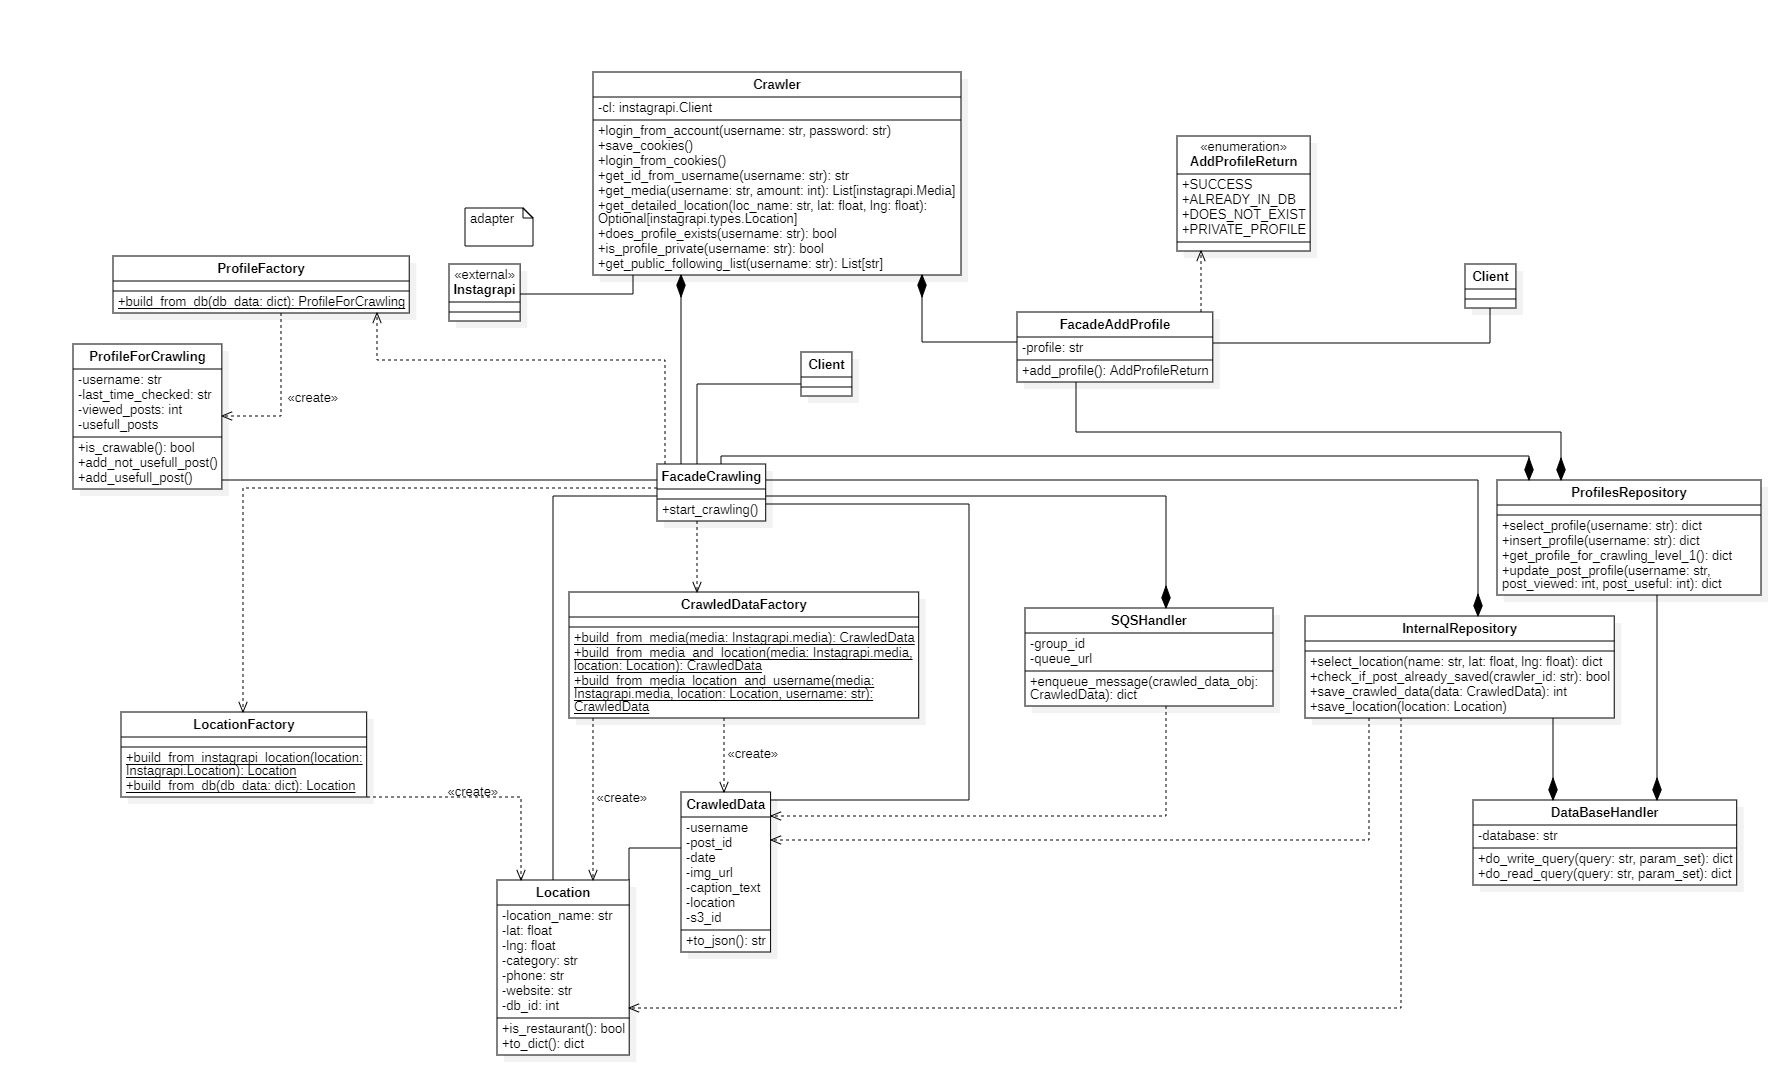
\includegraphics[scale=0.35]{Contenuto/Immagini/classi-CS.JPG}
    \caption{Crawling Service - Diagramma delle classi}
\end{figure}

\subsubsection{Diagrammi di sequenza}
\begin{figure}[!h]
    \centering
    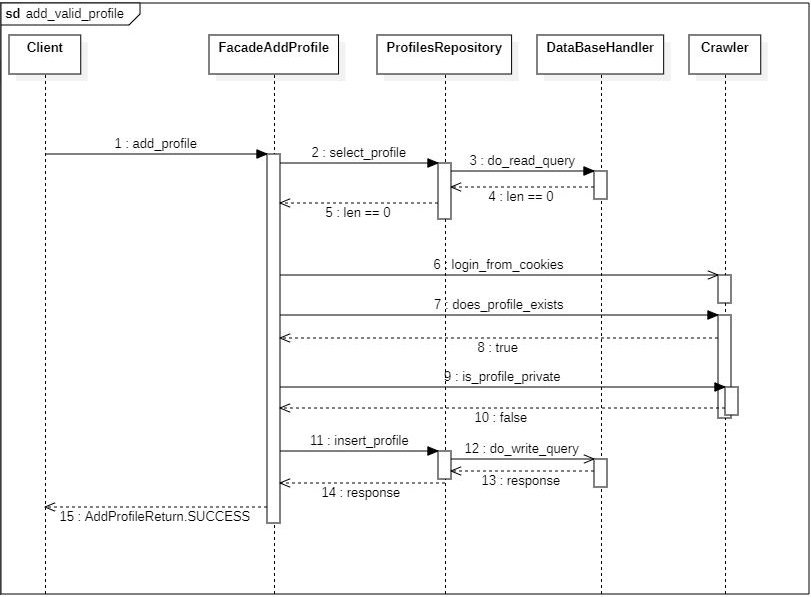
\includegraphics[scale=0.65]{Contenuto/Immagini/seq1-CS.JPG}
    \caption{Crawling Service - Diagramma di sequenza - 1}
\end{figure}
\begin{figure}[!h]
    \centering
    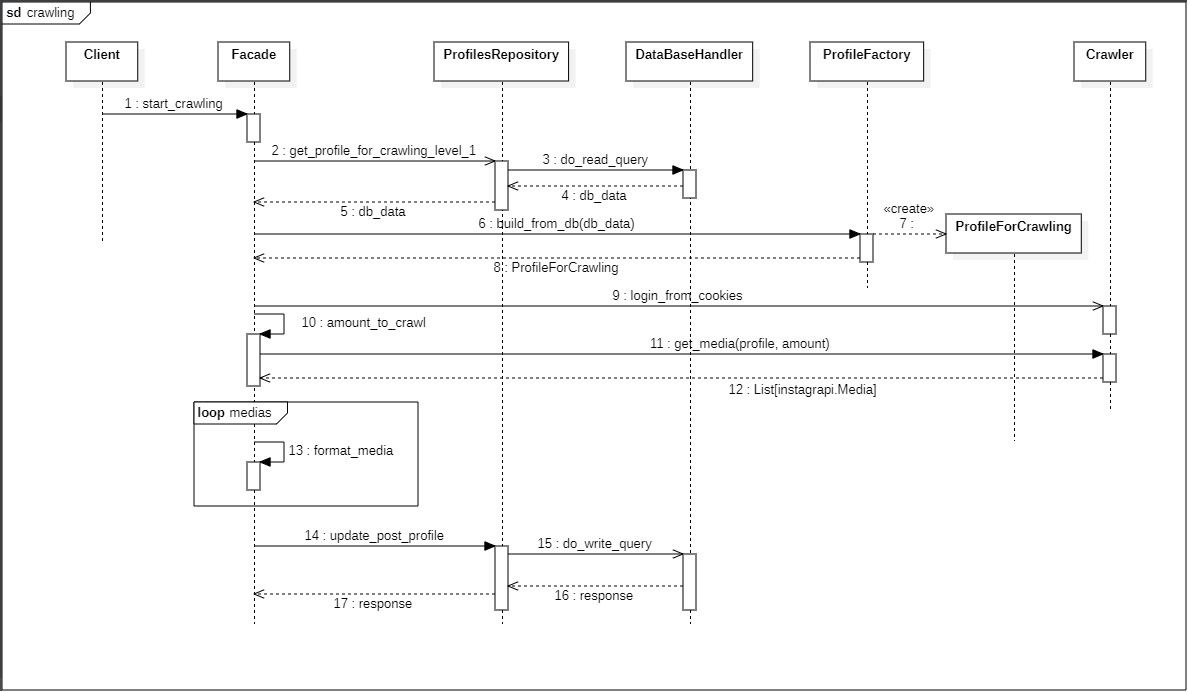
\includegraphics[scale=0.35]{Contenuto/Immagini/seq2-CS.JPG}
    \caption{Crawling Service - Diagramma di sequenza - 2}
\end{figure}
\begin{figure}[!h]
    \centering
    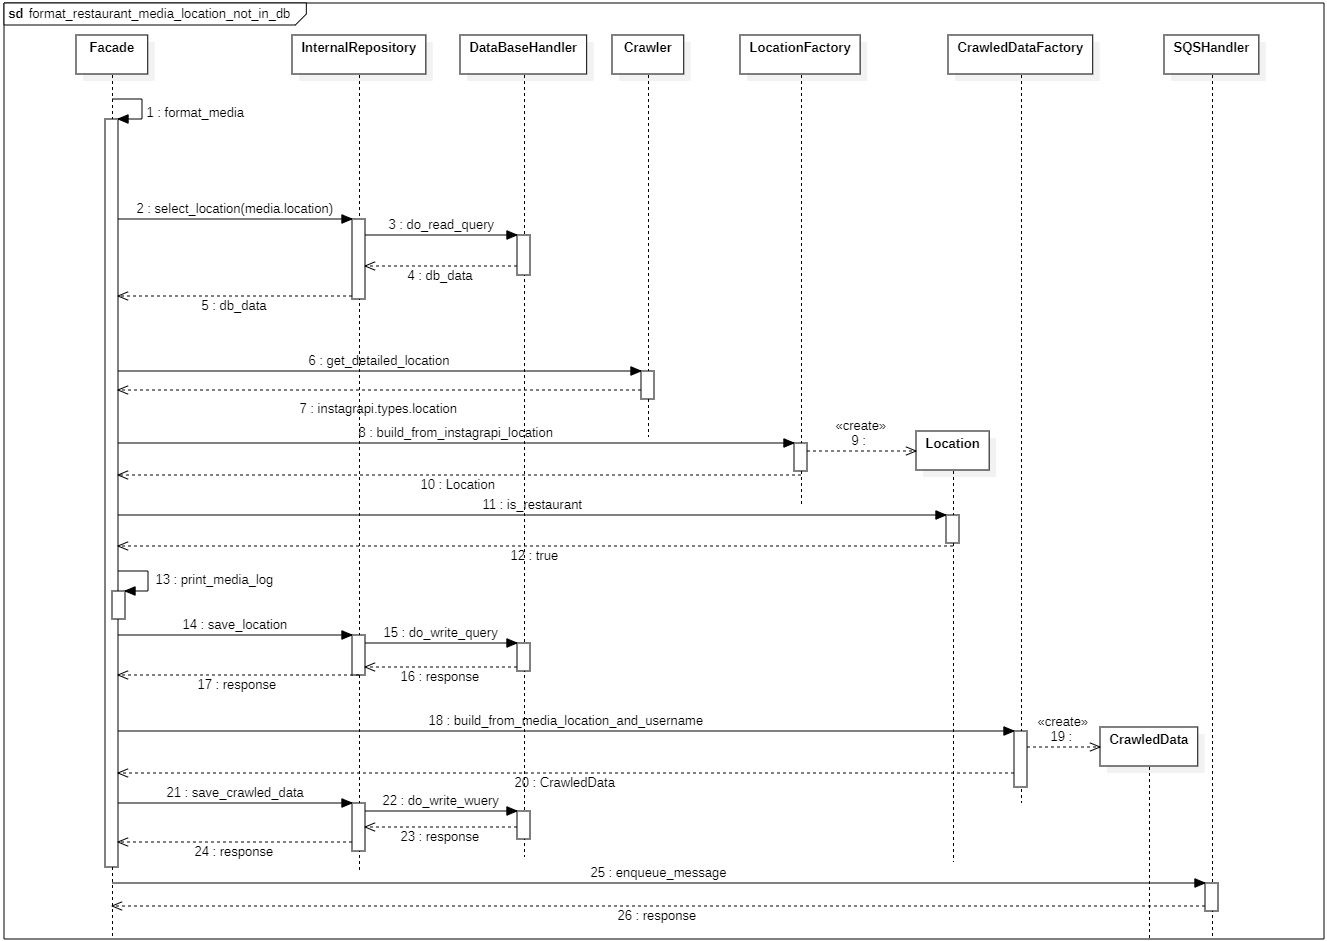
\includegraphics[scale=0.35]{Contenuto/Immagini/seq3-CS.JPG}
    \caption{Crawling Service - Diagramma di sequenza - 3}
\end{figure}

\subsubsection{Design pattern notevoli utilizzati}
Per La realizzazione del Crawling Service sono stati utilizzati i seguenti design pattern:
\begin{itemize}
    \item \textbf{Facade:} Utilizzato per la realizzazione delle classi FacadeCrawling e FacadeAddProfile, in modo da 
    \item \textbf{Adapter:}
    \item \textbf{Static Factory:}
\end{itemize}